

\tikzset{every picture/.style={line width=0.75pt}} %set default line width to 0.75pt        

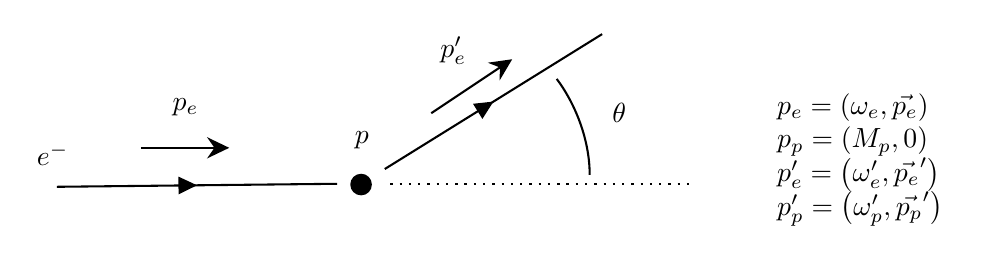
\begin{tikzpicture}[x=0.75pt,y=0.75pt,yscale=-1,xscale=1]
%uncomment if require: \path (0,300); %set diagram left start at 0, and has height of 300

%Straight Lines [id:da47004371895046315] 
\draw    (94,144.56) -- (229.06,143.11) ;
\draw [shift={(161.53,143.83)}, rotate = 539.39] [fill={rgb, 255:red, 0; green, 0; blue, 0 }  ][line width=0.08]  [draw opacity=0] (8.93,-4.29) -- (0,0) -- (8.93,4.29) -- cycle    ;
%Flowchart: Connector [id:dp08357812112166041] 
\draw  [fill={rgb, 255:red, 0; green, 0; blue, 0 }  ,fill opacity=1 ] (235.89,143.47) .. controls (235.89,146.06) and (237.99,148.17) .. (240.58,148.17) .. controls (243.18,148.17) and (245.28,146.06) .. (245.28,143.47) .. controls (245.28,140.88) and (243.18,138.78) .. (240.58,138.78) .. controls (237.99,138.78) and (235.89,140.88) .. (235.89,143.47) -- cycle ;
%Straight Lines [id:da8179679192746647] 
\draw    (252,136) -- (356.72,71) ;
\draw [shift={(304.36,103.5)}, rotate = 508.17] [fill={rgb, 255:red, 0; green, 0; blue, 0 }  ][line width=0.08]  [draw opacity=0] (8.93,-4.29) -- (0,0) -- (8.93,4.29) -- cycle    ;
%Straight Lines [id:da15056850292634993] 
\draw  [dash pattern={on 0.84pt off 2.51pt}]  (254.67,143.11) -- (399.83,143.11) ;
%Curve Lines [id:da5581541176414646] 
\draw    (334.83,92.56) .. controls (343.5,104.11) and (350.72,121.44) .. (350.72,138.78) ;
%Straight Lines [id:da452390952963887] 
\draw [line width=0.75]    (134.44,125.78) -- (174.06,125.78) ;
\draw [shift={(177.06,125.78)}, rotate = 180] [fill={rgb, 255:red, 0; green, 0; blue, 0 }  ][line width=0.08]  [draw opacity=0] (10.72,-5.15) -- (0,0) -- (10.72,5.15) -- (7.12,0) -- cycle    ;
%Straight Lines [id:da857484560177197] 
\draw [line width=0.75]    (274.39,109.11) -- (310.89,84.78) ;
\draw [shift={(313.39,83.11)}, rotate = 506.31] [fill={rgb, 255:red, 0; green, 0; blue, 0 }  ][line width=0.08]  [draw opacity=0] (10.72,-5.15) -- (0,0) -- (10.72,5.15) -- (7.12,0) -- cycle    ;

% Text Node
\draw (365,109) node    {$\theta $};
% Text Node
\draw (156,106) node    {$p_{e}$};
% Text Node
\draw (285,79) node    {$p_{e} '$};
% Text Node
\draw (92,129) node    {$e^{-}$};
% Text Node
\draw (241,122) node    {$\text{p}$};
% Text Node
\draw (481,131) node    {$ \begin{array}{l}
p_{e} =\left( \omega_{e} ,\vec{p_{e}}\right)\\
p_{p} =( M_{p} ,0)\\
p_{e} '=\left( \omega_{e} ',\vec{p_{e}} '\right)\\
p_{p} '=\left( \omega_{p} ',\vec{p_{p}} '\right)
\end{array}$};


\end{tikzpicture}